\part{Linear Programming}
	\chapter{Formulation}
		\section{Linear Programming Problem Manipulation}
			\subsection{Inequalities and Equalities}
				An inequality can be transformed into an equation by adding or subtracting the nonnegative slack or surplus variable
				\begin{equation}
					\sum_{j=1}^na_{ij}x_j \ge b_i \Rightarrow \sum_{j=1}^na_{ij}x_j - x_{n+1} = b_i 
				\end{equation}
				or
				\begin{equation}
					\sum_{j=1}^na_{ij}x_j \le b_i \Rightarrow \sum_{j=1}^na_{ij}x_j + x_{n+1} = b_i 
				\end{equation}
				Although it is not the practice, equality can be transformed into inequality too
				\begin{equation}
					\sum_{j=1}^na_{ij}x_j = b_i \Rightarrow \begin{cases}\sum_{j=1}^na_{ij}x_j \le b_i \\ \sum_{j=1}^na_{ij}x_j \ge b_i \end{cases} 
				\end{equation}
				Also, in linear programming, we only care about close set, so we will not have $<$, $>$ in the formulation, we can use the following
				\begin{equation}
					\sum_{j=1}^na_{ij}x_j > b_i \Rightarrow \sum_{j=1}^na_{ij}x_j \ge b_i + \epsilon 
				\end{equation}
				where $\epsilon$ is a small number.
			
			\subsection{Minimization and Maximization}
				To convert a minimization problem into a maximization problem, we can use the following to define a new objective function
				\begin{equation}
					\min \sum_{j=1}^nc_jx_j = -\max \sum_{j=1}^n c_jx_j 
				\end{equation}
			
			\subsection{Standard Form and Canonical Form}
				Standard Form
				\begin{align}
					\min \quad & \sum_{j=1}^nc_jx_j \\
					\text{s.t.} \quad & Ax = b \\
									  & x \ge 0 
				\end{align}
				Canonical Form
				\begin{align}
					\min \quad & \sum_{j=1}^nc_jx_j \\
					\text{s.t.} \quad & Ax \le b \\
									  & x \ge 0 
				\end{align}

		\section{Typical Problems}

		\section{Formulation Skills}
			\subsection{Absolute Value}
				Consider the following model statement:
				\begin{align}
					\min \quad & \sum_{j\in J}c_j|x_j|, \quad c_j > 0 \\
					\text{s.t.} \quad & \sum_{j\in J}a_{ij}x_j \gtreqless b_i, \quad \forall i\in I \\
					                  & x_j \quad \text{unrestricted}, \quad \forall j\in J 
				\end{align}
				Modeling:
				\begin{align}
					\min \quad & \sum_{j\in J}c_j(x_j^+ + x_j^-), \quad c_j > 0 \\
					\text{s.t.} \quad & \sum_{j\in J}a_{ij}(x_j^+ - x_j^-) \gtreqless b_i, \quad \forall i\in I \\
					                  & x_j^+, x_j^- \ge 0, \quad \forall j\in J 
				\end{align}

			\subsection{A Minimax Objective}
				Consider the following model statement:
				\begin{align}
					\min \quad & \max_{k\in K}\sum_{j\in J}c_{kj}x_j \\
					\text{s.t.} \quad & \sum_{j\in J}a_{ij}x_j \gtreqless b_i, \quad \forall i\in I \\
					                  & x_j \ge 0, \quad \forall j\in J 
				\end{align}
				Modeling:
				\begin{align}
					\min \quad & z \\
					\text{s.t.} \quad & \sum_{j\in J}a_{ij}x_j \gtreqless b_i, \quad \forall i\in I \\
									  & \sum_{j\in J}c_{kj}x_j \le z, \quad \forall k\in K \\
					                  & x_j \ge 0, \quad \forall j\in J 
				\end{align}
			\subsection{A fractional Objective}
				Consider the following model statement:
				\begin{align}
					\min \quad & \frac{\sum_{j\in J}c_{j}x_j + \alpha}{\sum_{j\in J}d_{j}x_j + \beta} \\
					\text{s.t.} \quad & \sum_{j\in J}a_{ij}x_j \gtreqless b_i, \quad \forall i\in I \\
					                  & x_j \ge 0, \quad \forall j\in J 
				\end{align}
				Modeling:
				\begin{align}
					\min \quad & \sum_{j\in J}c_{j}x_jt + \alpha t \\
					\text{s.t.} \quad & \sum_{j\in J}a_{ij}x_j \gtreqless b_i, \quad \forall i\in I \\
									  & \sum_{j\in J}d_jx_jt + \beta t = 1\\
									  & t > 0 \\
					                  & x_j \ge 0, \quad \forall j\in J \\
					                  & (t = \frac1{\sum_{j\in J}d_jx_j + \beta}) 
				\end{align}
			\subsection{A range Constraint}
				Consider the following model statement:
				\begin{align}
					\min \quad & \sum_{j\in J}c_jx_j \\
					\text{s.t.} \quad & d_i\le \sum_{j\in J}a_{ij}x_j \le e_i, \quad \forall i\in I \\
					                  & x_j \ge 0, \quad \forall j\in J 
				\end{align}
				Modeling:
				\begin{align}
					\min \quad & \sum_{j\in J}c_jx_j, \quad c_j > 0 \\
					\text{s.t.} \quad & u_i + \sum_{j\in J}a_{ij}x_j = e_i, \quad \forall i\in I \\
					                  & x_j \ge 0, \quad \forall j\in J \\
					                  & 0\le u_i \le e_i-d_i, \quad \forall i\in I 
				\end{align}

	\chapter{Simplex Method}
		\section{Basic Feasible Solutions and Extreme Points}
			\begin{definition}
				Consider the system $\{A_{m\times n}x=b_m, x\ge 0\}$, suppose $rank(A, b) = rank(A) =m$, we can arrange $A$ and have a partition of $A$. Let $A=[B, N]$ where $B$ is $m\times m$ invertible matrix, and $N$ is a $m\times (n-m)$ matrix. The solution $x=\left[\begin{matrix}x_B\\x_N\end{matrix}\right]$ to the equation $Ax=b$, where
				\begin{equation}
					x_B = B^{-1}b 
				\end{equation}
				and
				\begin{equation}
					x_N = 0 
				\end{equation}
				is called \textbf{basic solution} of system. If $x_B \ge 0$, it is called \textbf{basic feasible solution}. If $x_B > 0$ it is called \textbf{non-degenerate basic feasible solution}. For $x_B \ge 0$, if some $x_j = 0$, those components are called \textbf{degenerated basic feasible solution}.\\
				$B$ is called the \textbf{basic matrix}, $N$ is called \textbf{nonbasic matrix}				
			\end{definition}

			\begin{theorem}
				$x$ is an E.P. $\iff$ $x$ is a B.F.S
			\end{theorem}
			
			\begin{proof}
				First, Let $x$ be a B.F.S., Suppose $x=\lambda u + (1 - \lambda) v$, for $u, v \in S, \lambda \in (0, 1)$\\
				Let $I = \{i: x_i > 0\}$ Then\\
				- if $i \notin I$ then $x_i = 0$, which implies $u_i = v_i = 0$
				- $\because Au = Av = b$, $\therefore A(u-v) = 0 \Rightarrow \sum_{i=1}^n(u_i - v_i)a_i = 0$, $\because u_i = v_i = 0$, for $i\notin I$, it implies $u_i = v_i$ for $i\in I$, Hence $u=v$, $x$ is E.P.\\
				Second, suppose $x$ is not B.F.S., i.e. $\{a_i: i \in I\}$ are linearly dependent.\\
				Then there $\exists u\ne 0, u_i =0 , i\notin I$ such that $Au=0$.\\
				Hence, for a small $\epsilon$, $x=\frac12(x + \epsilon u) + \frac12(x - \epsilon u)$, $x$ is not E.P.					
			\end{proof}

		\section{Simplex Method}
			\subsection{Key to Simplex Method}
				\subsubsection{Cost Coefficient}
					The cost coefficient can be derived from the following
					\begin{align}
						z &= cx \\
						  &= c_Bx_B + c_Nx_N \\
						  &= c_B(B^{-1}b - B^{-1}Nx_N) + c_Nx_N\\
						  &= c_BB^{-1}b - \sum_{j\in N}(c_BB^{-1}a_j - c_j)x_j \\
						  &= c_BB^{-1}b - \sum_{j\in N}(z_j-c_j)x_j 
 					\end{align}
 					We denote $z_0 = c_BB^{-1}b$, $z_j = c_B^{-1}a_j$, $\bar{b} = B^{-1}b$ and $y_j = B^{-1}a_j$ for all nonbasic variables.\\
 					The formulation can be transformed into
 					\begin{align}
 						\min \quad & z = z_0 - \sum_{j\in N}(z_j - c_j)x_j\\
 						\text{s.t.} \quad & \sum_{j\in N}y_jx_j + x_B = \bar{b} \\
 										  & x_j \ge 0, j\in N \\
 										  & x_B \ge 0 
 					\end{align}
 					In the above formulation, $z_j - c_j$ is the cost coefficient. If $\exists j$ and $z_j - c_j > 0$, it means the objective function can still be optimized. (If $\forall j$, $z_j - c_j \le 0$, then $z \ge z_0$ for any feasible solution, $z$ is the optimal solution)

 				\subsubsection{Pivot}
 					After finding the most violated $z_j - c_j$, we find a variable, say $x_k$, where $z_k - c_k = \min \{z_j - c_j\}$ to be the variable leaving the basis. \\
 					If there are degenerated variables, we can perform different method to choose variable to enter basis.

 				\subsubsection{Minimum Ratio}
 					\begin{equation}
 						x_{B_i} = \bar{b}_i - y_{ik}x_k \ge 0 
 					\end{equation}
 					Therefore we have the minimum ratio rule
 					\begin{equation}
 						x_k = \min_{i \in B} \{\frac{\bar{b}_i}{y_{ik}}, y_{ik} > 0\} 
 					\end{equation}
 					If for the that column all $y_{ik} \le 0$, unbounded.

			\subsection{Simplex Method Algorithm}
				The pseudo-code of Simplex Method is given as following:
				\begin{algorithm}[h!]
					\caption{Simplex Method}
					\begin{algorithmic}[1]
						\REQUIRE Given a basic feasible solution with basis $B$
						\ENSURE Optimal objective value $\min z= cx$
						\STATE Set $\mathbf{B}$ for basic variables, $\mathbf{N}$ for nonbasic variables
						\STATE $\mathbf{B} \gets \text{all slack variables}$
						\STATE $\mathbf{N} \gets \text{all variables excepts slack variables}$
						\FOR{$\forall j$}
							\STATE $z_j=c_BB^{-1}a_j=0$				
						\ENDFOR
						\WHILE{$\exists z_j-c_j > 0$}
							\STATE $z_j=wa_j-c_j=c_BB^{-1}a_j-c_j$
							\STATE $z_k-c_k=\max\limits_{j \in \mathbf{N}}\{z_j-c_j\}$
							\STATE $y_k=B^{-1}a_k$
							\IF{$\exists y_{ik} >0$}
								\STATE $\theta_r=\min\limits_{i \in \mathbf{B}}\{\theta_i=\frac{\bar{b}_i}{y_{ik}}:y_{ik}>0\}$
								\STATE $\mathbf{B} \gets \mathbf{B} \backslash \{k\}$
								\STATE $\mathbf{N} \gets \mathbf{N} \cup \{k\}$
								\STATE $\mathbf{B} \gets \mathbf{B} \cup \{r\}$
								\STATE $\mathbf{N} \gets \mathbf{N} \backslash \{r\}$
							\ELSE
								\STATE Unbounded
							\ENDIF
						\ENDWHILE
						\STATE $x_B^*=B^{-1}b=\bar{b}$
						\STATE $x_N=0$
						\STATE $z^*=c_BB^{-1}b=c_B\bar{b}\mathbf{a_{B_k}}$
					\end{algorithmic}
				\end{algorithm}

		\section{Find Elements in Tableau}
				Initial tableau:\\
				\begin{align}
					\begin{tabular} {|c|c|c|c|c|c|c|c|}
						\hline
						& $z$ & $x_1$ & $x_2$ & $x_3$ & $x_4$ & $x_5$ & RHS \\
						\hline
						$z$ & 1 & 1 & 3 & 0 & 0 & 0 & 0 \\
						\hline
						$x_3$ & 0 & 1 & -2 & 1 & 0 & 0 & 0 \\
						\hline
						$x_4$ & 0 & -2 & \framebox{1} & 0 & 1 & 0 & 4\\
						\hline
						$x_5$ & 0 & 5 & 3 & 0 & 0 & 1 & 15 \\
						\hline
					\end{tabular}
				\end{align}
				Last tableau:\\
				\begin{align}
					\begin{tabular} {|c|c|c|c|c|c|c|c|}
						\hline
						& $z$ & $x_1$ & $x_2$ & $x_3$ & $x_4$ & $x_5$ & RHS \\
						\hline
						$z$ & 1 & 0 & 0 & 0 & $-\frac{12}{11}$ & $-\frac{7}{11}$ & $-\frac{153}{11}$ \\
						\hline
						$x_3$ & 0 & 0 & 1 & 1 & $\frac{13}{11}$ & $\frac{3}{11}$ & $\frac{97}{11}$ \\
						\hline
						$x_2$ & 0 & 1 & 0 & 0 & $\frac{5}{11}$ & $\frac{2}{11}$ & $\frac{50}{11}$ \\
						\hline
						$x_1$ & 1 & 0 & 0 & 0 & $-\frac{3}{11}$ & $\frac{1}{11}$ & $\frac{3}{11}$ \\
						\hline
					\end{tabular}
				\end{align}
				- The optimal basic variables are $x_3$, $x_2$, $x_1$. The optimal basis is the columns in the initial tableau with correspond columns
				\begin{equation}
					B = \left(\begin{matrix}
						\frac{13}{11} & \frac{3}{11} & \frac{97}{11}\\
						\frac{5}{11} & \frac{2}{11} & \frac{50}{11}\\
						-\frac{3}{11} & \frac{1}{11} & \frac{3}{11}\\
					\end{matrix}\right)
				\end{equation}
				- From the initial tableau, we can see the initial basis is built from slack variables $x_3$, $x_4$, $x_5$. The $B^{-1}$ is the correspond columns in final tableau.
				\begin{equation}
					B = \left(\begin{matrix}
						1 & -2 & 1\\
						0 & 1 & -2\\
						0 & 3 & 5\\
					\end{matrix}\right) 		
				\end{equation}
				- The optimal basic variables are $x_3$, $x_2$, $x_1$. Find $c_B$ in the initial tableau.
				\begin{equation}
					c_B = \left(\begin{matrix}
						0\\3\\1
					\end{matrix}\right) 
				\end{equation}
				- Find $w=c_BB^{-1}$ from the final tableau, correspond to the slack variable.
				\begin{equation}
					w = c_BB^{-1} = \left(\begin{matrix}
						0\\-\frac{12}{11}\\-\frac7{11}
					\end{matrix}\right) 
				\end{equation}

		\section{Artificial Variable}
			If some of the constraint is not in $\sum_{i=1}^na_ix_i \le 0$ form, we cannot add a positive slack variable. In this case, we add an artificial variable other than slack variable.
			\begin{equation}
				\sum_{i=1}^n a_ix_i \ge (or =) 0 \Rightarrow \sum_{j=1}^n a_ix_i + x_a = 0 
			\end{equation}
			Notice that in an optimal solution, $x_a = 0$, otherwise it is not valid.\\
			Artificial variables are only a tool to get the simplex method started.
			\subsection{Two-Phase Method}
				\subsubsection{Two-Phase Method}
					For \textbf{Phase I:}\\
						Solve the following program start with a basic feasible solution $x=0, x_a=b$, i.e., the artificial variable forms the basis.
						\begin{align}
							\min \quad & 1x_a \\
							\text{s.t.} \quad & Ax + x_a = b \\
											  & x \ge 0 \\
											  & x_a \ge 0 
						\end{align}
						If the optimal $1x_a \ne 0$, infeasible, stop. Otherwise proceed Phase II.
					For \textbf{Phase II:}\\
						Remove the columns of artificial variables, replace the objective function with the original objective function, proceed to solve simplex method.
				\subsubsection{Discussion}
					\textbf{Case A:} $x_a \ne 0$\\
						Infeasible.\\
					\textbf{Case B.1:} $x_a = 0$ and all artificial variables are out of the basis\\
					At the end of Phase I, we derive
					\begin{align}
						\begin{tabular} {|c|c|c|c|c|}
							\hline
							$x_0$ & $x_B$ & $x_N$ & $x_a$ & RHS \\
							\hline
							1 & 0 & 0 & -1 & 0\\
							\hline
							0 & $I$ & $B^{-1}N$ & $B^{-1}$ & $B^{-1}b$ \\
							\hline
						\end{tabular} 
					\end{align}
					We can discard $x_a$ columns, (or we can leave it because it keeps track of $B^{-1}$), and then we do the Phase II
					\begin{align}
						\begin{tabular} {|c|c|c|c|}
							\hline
							$z$ & $x_B$ & $x_N$ & $RHS$ \\
							\hline
							1 & 0 & $c_BB^{-1}N - c_N$ & $c_BB^{-1}b$ \\
							\hline
							0 & $I$ & $B^{-1}N$ & $B^{-1}b$ \\
							\hline
						\end{tabular} 		
					\end{align}
					\textbf{Case B.2:} Some artificial variables are in the basis at zero values\\
					This is because of degeneracy. We pivot on those artificial variables, once they leave the basis, eliminate them.
			\subsection{Big M Method}

			\subsection{Single Artificial Variable}

		\section{Revised Simplex Method}
			\subsection{Key to Revised Simplex Method}
				The procedure of Simplex Method is (almost) exactly the same as original simplex method. However, notice that we don't need to use $N$ so for the revised simplex method, we don't calculate any matrix related to $N$\\
				The original matrix:
				\begin{align}
					\begin{tabular} {|c|c|c|c|}
						\hline
						$z$ & $x_B$ & $x_N$ & $RHS$ \\
						\hline
						1 & 0 & $c_BB^{-1}N - c_N$ & $c_BB^{-1}b$ \\
						\hline
						0 & $I$ & $B^{-1}N$ & $B^{-1}b$ \\
						\hline
					\end{tabular} 		
				\end{align}
				The revised matrix:
				\begin{align}
					\begin{tabular} {|c|c|}
						\hline
						Basic Inverse & RHS \\
						\hline
						$w=c_BB^{-1}$ & $c_B\bar{b} = c_BB^{-1}b$\\
						\hline
						$B^{-1}$ & $\bar{b} = B^{-1}b$\\
						\hline
					\end{tabular} 
				\end{align}
				For each pivot iteration, calculate $z_j - c_j = wa_j - c_j = c_BB^{-1}a_j - c_j, \forall j\in N$, pivot rules are the same as simplex method, each time find a variable $x_k$ to enter basis
				\begin{align}
					\begin{tabular}{|c|c|c|c|}
						\cline{1-2} \cline{4-4} $B^{-1}$ & RHS & & $x_k$ \\
						\cline{1-2} \cline{4-4} $w$ & $c_B\bar{b}$ & & $z_k-c_k$ \\
						\cline{1-2} \cline{4-4} $B^{-1}$ & $\bar{b}$ & & $y_k$ \\
						\cline{1-2} \cline{4-4}
					\end{tabular} 
				\end{align}
				Do the minimum ratio rule to find the variable $x_r$ to leave the basis
				\begin{align}
					\begin{tabular}{|c|c|c|c|}
						\cline{1-2} \cline{4-4} $B^{-1}$ & RHS & & $x_k$ \\
						\cline{1-2} \cline{4-4} $w$ & $c_B\bar{b}$ & & $z_k-c_k$ \\
						\cline{1-2} \cline{4-4} & $\bar{b_1}$ & & $y_{1k}$\\
						& $\bar{b_2}$ & & $y_{2k}$\\
						& ... & & ...\\
						$B^{-1}$ & $\bar{b_r}$ & & $y_{rk}$(pivot at here)\\
						& ... & & ...\\
						& $\bar{b_m}$ & & $y_{mk}$\\
						\cline{1-2} \cline{4-4} 
					\end{tabular}
				\end{align}

			\subsection{Comparison between Simplex and Revised Simplex}
				\subsubsection{Advantage of Revised Simplex}
				- Save storage memory \\
				- Don\rq{}t need to calculate N (including $B^{-1}N$ and $c_BB^{-1}N$) \\
				- More accurate because round up errors will not be accumulated 

				\subsubsection{Disadvantage of Revised Simplex}
				- Need to calculate $wa_j$ for all $j \in N$ (in fact don\rq{}t need to calculated it for the variable just left the basis) 

				\subsubsection{Computation Complexity}
				\begin{align}
					\begin{tabular}{|c|c|c|}
						\hline Method & Type & Operations\\
						\hline Simplex & $\times$ & $(m+1)(n-m+1)$\\
						\cline{2-3} & $+$ & $m(n-m+1)$\\
						\hline Revised Simplex & $\times$ & $(m+1)^2+m(n-m)$ \\
						\cline{2-3} & $+$ & $m(m+1)+m(n-m)$ \\
						\hline
					\end{tabular} 
				\end{align}

				\subsubsection{When to use?}
				- When $m >> n$, do revise simplex method on the dual problem \\
				- When $m \simeq n$, revise simplex method is not as good as simplex method \\
				- When $m << n$ perfect for revise simplex method.
				
			\subsection{Decomposition of B inverse}
				Let $B=\{ a_{B_1}, a_{B_2}, ..., a_{B_r}, ..., a_{B_m}\}$ and $B^{-1}$ is known.
				If $a_{B_r}$ is replaced by $a_{B_k}$, then $B$ becomes $\bar{B}$. Which means $a_{B_r}$ enters the basis and $a_{B_k}$ leaves the basis. \\
				Then $\bar{B}^{-1}$ can be represent by $B^{-1}$. Noting that $a_k=By_k$ and $a_{B_i}=Be_i$, then
				\begin{align}
					\bar{B} & = (a_{B_1}, a_{B_2}, ...,a_{B_{r-1}}, a_k, a_{B_{r+1}}, a_m)  \\
					& = (Be_1, Be_2, ..., Be_{r-1}, By_k, Be_{r+1}, ..., Be_m)  \\
					& = BT 
				\end{align}
				where $T$ is
				\begin{equation}
					T=\left[ \begin{array}{cccccccc}
						1 & 0 & ... & 0 & y_{1k} & 0 & ... & 0 \\
						0 & 1 & ... & 0 &  y_{2k} & 0 & ... & 0 \\
						\vdots & \vdots & & \vdots & \vdots & \vdots & & \vdots \\
						0 & 0 & ... & 1 & y_{r-1,k} & 0 & ... & 0 \\
						0 & 0 & ... & 0 & y_{rk} & 0 & ... & 0 \\
						0 & 0 & ... & 0 &  y_{r+1,k} & 1 & ... & 0 \\
						\vdots & \vdots & & \vdots & \vdots & \vdots & & \vdots \\
						0 & 0 & ... & 0 &  y_{mk}& 0 & ... & 1 \\
					\end{array} \right] 
				\end{equation}
				and 
				\begin{equation}
					E =  T ^{-1}=\left[ \begin{array}{cccccccc}
						1 & 0 & ... & 0 & \frac{-y_{1k}}{y_{rk}} & 0 & ... & 0 \\
						0 & 1 & ... & 0 & \frac{-y_{2k}}{y_{rk}} & 0 & ... & 0 \\
						\vdots & \vdots & & \vdots & \vdots & \vdots & & \vdots \\
						0 & 0 & ... & 1 & \frac{-y_{r-1,k}}{y_{rk}} & 0 & ... & 0 \\
						0 & 0 & ... & 0 & \frac{1}{y_{rk}} & 0 & ... & 0 \\
						0 & 0 & ... & 0 & \frac{-y_{r+1,k}}{y_{rk}} & 1 & ... & 0 \\
						\vdots & \vdots & & \vdots & \vdots & \vdots & & \vdots \\
						0 & 0 & ... & 0 &  \frac{-y_{mk}}{y_{rk}} & 0 & ... & 1 \\
					\end{array} \right] 
				\end{equation}
				For each iteration, i.e. one variable enters the basis and one leaves the basis, $\bar{B}^{-1}=T^{-1}B^{-1}=EB^{-1}$. Given that the first iteration starts from slack variables, the first basis $B_1$ is $I$, then we have
				\begin{equation}
					B^{-1}_t=E_{t-1} E_{t-2} \cdots E_{2} E_{1} I
				\end{equation}
				Using $E$ in calculation can simplify the product of matrix where
				\begin{align}
					cE &= {c_1,c_2,...,c_m} \left[ \begin{array}{cccccc}
					1 & 0 & ... & g_1 & ... & 0 \\
					0 & 1 & ... & g_2 & ... & 0 \\
					\vdots & \vdots & & \vdots & & \vdots \\
					0 & 0 & ... & g_m & ... & 1 \\
					\end{array} \right]  \\
					&= (c_1, c_2, ... ,c_{r-1}, cg, c_{r+1}, ..., c_m) 
				\end{align}
				and
				\begin{align}
					Ea &=  \left[ \begin{array}{cccccc}
					1 & 0 & ... & g_1 & ... & 0 \\
					0 & 1 & ... & g_2 & ... & 0 \\
					\vdots & \vdots & & \vdots & & \vdots \\
					0 & 0 & ... & g_m & ... & 1 \\
					\end{array} \right]
					 \left[ \begin{array}{c}
					a_1 \\
					a_2 \\
					\vdots \\
					a_m \\
					\end{array} \right]  \\
					&= 
					\left[ \begin{array}{c}
					a_1 \\
					a_2 \\
					\vdots \\
					a_{r-1} \\
					0 \\
					a_{r+1} \\
					\vdots \\
					a_m \\
					\end{array} \right] +
					a_r\left[ \begin{array}{c}
					g_1 \\
					g_2 \\
					\vdots \\
					g_{r-1} \\
					g_r \\
					g_{r+1} \\
					\vdots \\
					g_m \\
					\end{array} \right]  \\
					&=\bar{a}+a_rg 
				\end{align}
				Then we can calculate $w$, $y_k$ and $\bar{b}$
				\begin{align}
					w&=c_BB^{-1} = c_BE_{t-1}E_{t-2}...E_2E_1  \\
					y_k &=B^{-1}a_k = E_{t-1}E_{t-2}...E_2E_1a_k  \\
					\bar{b}&=B^{-1}_{t+1}b=E_tE_{t-1}E_{t-2}...E_2E_1b 
				\end{align}

		\section{Simplex for Bounded Variables}
			\subsection{Bounded Variable Formulation}
				\begin{align}
					\min \quad & cx \\
					\text{s.t.} \quad & Ax=b \\
									  & l \le x\le b 
				\end{align}
				Reason why we don't the following formulation
				\begin{align}
					\min \quad & cx \\
					\text{s.t.} \quad & Ax=b \\
					                  & x - Ix_l = l \\
					                  & x + Ix_u = u \\
					                  & x \ge 0\\
					                  & x_l \ge 0\\
					                  & x_u \ge 0 
				\end{align}
				is that this formulation increase the number of variable from $n$ to $3n$, and the number of constraint from $m$ to $m+2n$, the size in increase significantly.

			\subsection{Basic Feasible Solution}
				Consider the system $Ax=b$ and $l\le x\le b$, where $A$ is a $m\times n$ matrix of rank $m$, the solution $\bar{x}$ is a \textbf{basic feasible solution} if $A$ can be partition into $[B, N_l, N_u]$ where the solution $x$ can be partition into $x=(x_B, x_{N_l}, x_{N_u})$, in which $\bar{x}_{N_l} = l_{N_l}$ and $\bar{x}_{N_u} = u_{N_u}$, therefore
				\begin{equation}
					\bar{x}_B = B^{-1}b - B^{-1}N_lx_{N_l} - B^{-1}N_ux_{N_u} 
				\end{equation}
				Furthermore, similar to definition of nonnegative variables, if $l_B \le x_B \le u_B$, $x_B$ is a basic feasible solution, if $l_B < x_B < u_B$, $x_B$ is a non-degenerate basic feasible solution. 

			\subsection{Improving Basic Feasible Solution}
				The basic variables and the objective function can be derived as following:
				\begin{align}
					x_B &= B^{-1}b - B^{-1}N_lx_{N_l} - B^{-1}N_ux_{N_u} \\
					  z &= c_Bx_B + c_{N_l}x_{N_l} + c_{N_u}x_{N_u} \\
					  	&= c_B(B^{-1}b - B^{-1}N_lx_{N_l} - B^{-1}N_ux_{N_u})  \\
					  	& \quad + c_Bx_B + c_{N_l}x_{N_l} + c_{N_u}x_{N_u}\\
					  	&= c_BB^{-1}b + (c_{N_l} - c_BB^{-1}N_l)x_{N_l} \\
					  	& \quad + (c_{N_u} - c_BB^{-1}N_u)x_{N_u} \\
					  	&= c_BB^{-1}b - \sum_{j \in J_1}(z_j - c_j)x_j - \sum_{j \in J_2}(z_j - c_j)x_j
				\end{align}
				$J_1$ is the set of variables at lower bound, $J_2$ is the set of the variables at upper bound.\\
				Notice that the right-hand-side no longer provide $c_BB^{-1}b$ and $B^{-1}b$. For the variable entering the basis, find the variable with
				\begin{equation}
					\max\{\max_{j\in J_1}\{z_j - c_j\}, \max_{j\in J_2}\{c_j - z_j\}\} 
				\end{equation}
				to enter the basis\\
				\framebox{\textbf{Tip:}} "Most violated rule"\\
				The minimum ratio rule is revised for bounded simplex
				\begin{align}
					\Delta &= \min \{\gamma_1, \gamma_2, u_k-l_k\} \\
					\gamma_1 &= \begin{cases}
									\min_{r\in J_1}\{\frac{\bar{b}_r-l_{B_r}}{y_{rk}}:y_{rk} > 0\} \\
									\min_{r\in J_2}\{\frac{\bar{b}_r-l_{B_r}}{-y_{rk}}:y_{rk} < 0\} \\
									\infty
								\end{cases} \\
					\gamma_2 &= \begin{cases}
									\min_{r\in J_1}\{\frac{u_{B_r} - \bar{b}_r}{-y_{rk}}:y_{rk} < 0\} \\
									\min_{r\in J_2}\{\frac{u_{B_r} - \bar{b}_r}{y_{rk}}:y_{rk} > 0\} \\
									\infty
								\end{cases} 
				\end{align}
				\framebox{\textbf{Tip:}}\\
				Use $l \le x+\Delta \le u$ to test the range of $\delta$, if it hits lower bound, it is called $\gamma_1$, if it hits upper bound, it is called $\gamma_2$.

		\section{Degeneracy and Cycling}
			\subsection{Degeneracy}
				\subsubsection{Degeneracy in Simplex Method}
					If the basic variable $x_B$ is not strictly $> 0$, i.e. if some basic variable equals to 0, we call it degenerate.

				\subsubsection{Degeneracy for Bounded Variables}
					If some basic variables are at their upper bound or lower bound, we call it degenerate.

			\subsection{Cycling}
				In the degenerate case, pivoting by the simplex rule does not always give a strict decrease in the objective function value, because it may have $b_r = 0$. It is possible that the tableau may repeat if we use the simplex rule.\\
				Geometrically speaking, it means that at the same point - extreme point - it corresponds to more than one feasible solutions, so when we are pivoting, we stays at the same place.\\
				In computer algorithm, we rarely care about cycling because the data in computer is not precise, it is very hard to get into cycling.

			\subsection{Cycling Prevent}
				\subsubsection{Lexicographic Rule}
					- For entering variable, same as simplex rule\\
					- For leaving variable, if there is a tie, choose the variable with the smallest $\frac{y_{r1}}{y_{rk}}$.

				\subsubsection{Bland's Rule}
					- For entering variable, choose the variable with smallest index where $z_j - c_j \le 0$\\
					- For leaving variable, if there is a tie, choose the variable with smallest index.

				\subsubsection{Successive Ratio Rule}
					- Select the pivot column as any column $k$ where $z_k - c_k \le 0$\\
					- Given $k$, select the pivot row $r$ as the minimum successive ratio row associated with column $k$.\\
					In other words, for pivot columns where there is no tie in the usual minimum ratio, the successive ratio rule reduces to the simplex rule

		\section{Dual Simplex Method}
			Maintain dual feasibility, i.e. primal optimality, and complementary slackness and work towards primal feasibility.
			\framebox{\textbf{Tip:}}The RHS become new $z_j - c_j$, the old $z_j - c_j$ become new RHS. We are actually solving the dual problem.

		\section{As a Search Algorithm}
			\subsection{Improving Search Algorithm}
				A simplex method is a search algorithm, for each iteration it finds a not-worse solution, which can be represented as:\\
				\begin{equation}x^t = x^{t-1}+\lambda_{t-1}d^{t-1}  \end{equation}
				Where\\
				- $x^t$ is the solution of the $t$th iteration\\
				- $\lambda_t$ is the step length of $t$th iteration\\
				- $d^t$ is the direction of the $t$th iteration\\
				For each iteration, it contains three steps:\\
				- Optimality test\\
				- Find direction\\
				- Find the step length
				
			\subsection{Optimality Test}
				\begin{align}
					z &= cx \\
					& = \left[\begin{matrix}c_B & c_N\end{matrix} \right] \left [ \begin{matrix}x_B \\ x_N \end{matrix} \right]  \\
					& = c_B x_B + c_N x_N  \\
				\text{and} \because &Ax=b  \\
					\therefore & Bx_B + Nx_N = b, x_B\ge 0, x_N\ge 0 \\
					\therefore & x_B = B^{-1}b-B^{-1}Nx_N \\
					z &= c_BB^{-1}b-c_BB^{-1}Nx_N+c_Nx_N
				\end{align}
				for current solution $\hat{x}=\left [\begin{matrix}\hat{x_B} \\ 0\end{matrix}\right]$, $\hat{z} = c_BB^{-1}b$, then
				\begin{equation}
					z - \hat{z} = \left[\begin{matrix}0 & c_N - c_BB^{-1}N \end{matrix} \right] \left[ \begin{matrix}x_B \\ x_N \end{matrix}\right] 
				\end{equation}
				The $c_N - c_BB^{-1}N$ is the reduced cost, for a minimized problem, if $c_N - c_BB^{-1}N > 0$ means $z - \hat{z} \ge 0$, it reaches the optimality because we cannot find a solution less than $\hat{z}$.\\
							
			\subsection{Find Direction}
				Suppose we choose $x_k$ as a candidate to pivot into Basis\\
				\begin{equation}
					x = \left[ \begin{matrix}B^{-1}b-B^{-1}a_kx_k \\ 0+e_kx_k\end{matrix}\right]=\left[ \begin{matrix}B^{-1}b \\ 0\end{matrix} \right] + \left[ \begin{matrix} -B^{-1}a_k \\ e_k \end{matrix} \right]x_k 
				\end{equation}
				In this form, we can see: $x$ is the result after $t$th iteration, $\left[ \begin{matrix}B^{-1}b \\ 0\end{matrix} \right]$ is the result after $(t-1)$th iteration. $ \left[ \begin{matrix} -B^{-1}a_k \\ e_k \end{matrix} \right]$ is the iteration direction, $x_k$ is the step length.\\
				The only requirement of $x_k$ is $r_k < 0$ where $r_k=c_k - z_k$ is reduce cost, which is the $k$th entry of $c_N - c_BB^{-1}N$. \\
				Generally speaking, we usually take $r_k = \min\{c_j - z_j\}$ (which in fact can not guarantee the efficient of the algorithm.)

			\subsection{Find the Step Length}
				We need to guarantee the non-negativity, so for each iteration, we need to make sure $x\ge 0$. Which means\\
				\begin{equation}B^{-1}b-B^{-1}a_kx_k \ge 0  \end{equation}
				Denote $B^{-1}b$ as $\bar{b}$, denote $B^{-1}a_k$ as $y_k$\\
				If $y_k \le 0$, we can have $x_k$ as large as infinite, which means unboundedness. \\
				If $y_k > 0$ now we can use the minimum ratio to guarantee non-negativity.\\
				\textbf{Remember} hit the bound, basic variable leave the basis and become non-basic variable.
			\subsection{Simplex Method Algorithm}

			\subsection{Simplex Method Tableau}

			\subsection{Simplex Method as a Search Algorithm}

	\chapter{Duality, Sensitivity and Relaxation}
		\section{Duality}
			\subsection{Dual Formulation}
				For any prime problem
				\begin{align}
					\text{min} \quad & cx \\
					\text{s.t.} \quad & Ax\ge b \\
								& x\ge 0 
				\end{align}
				we can have a dual problem
				\begin{align}
					\text{max} \quad & wb  \\
					\text{s.t.} \quad & wA\le c\\
								& w \ge 0
				\end{align}
				
			\subsection{Mixed Forms of Duality}
				For the following prime problem
				\begin{align}
					\text{P(or D)} \quad \min \quad & c_1x_1 + c_2x_2 + c_3x_3 \\
					\quad \text{s.t.} \quad & A_{11}x_1 + A_{12}x_2 + A_{13}x_3 \ge b_1 \\
											& A_{21}x_1 + A_{22}x_2 + A_{23}x_3 \le b_2 \\
											& A_{31}x_1 + A_{32}x_2 + A_{33}x_3 = b_3 \\
											& x_1 \ge 0 \\
											& x_2 \le 0 \\
											& x_3 \quad \text{unrestricted} 
				\end{align}
				The dual of the problem
				\begin{align}
					\text{D(or P)} \quad \max \quad & w_1b_1 + w_2b_2 + w_3b3 \\
					\quad \text{s.t.} \quad & w_1A_{11} + w_2A_{21} + w_3A_{31} \le c_1 \\
											& w_1A_{12} + w_2A_{22} + w_3A_{32} \ge c_2 \\
											& w_1A_{13} + w_2A_{23} + w_3A_{33} = c_3 \\
											& w_1 \ge 0 \\
											& w_2 \le 0 \\
											& w_3 \quad \text{unrestricted} 
				\end{align}
				In sum, the relation between primal and dual problems are listed as following\\
				\begin{tabular}{|c|c|c|c|c|}
					\hline & Minimization& & Maximization& \\
					\hline & $\geq 0$ & $\longleftrightarrow$ & $\leq 0$ & \\
					Var & $\leq 0$ & $\longleftrightarrow$ & $\geq 0$ & Cons \\
					& Unrestricted & $\longleftrightarrow$ & = & \\
					\hline & $\geq 0$ & $\longleftrightarrow$ & $\geq 0$ & \\
					Cons & $\leq 0$ & $\longleftrightarrow$ & $\leq 0$ & Var \\
					& = & $\longleftrightarrow$ & Unrestricted & \\
					\hline
				\end{tabular} 

			\subsection{Dual of the Dual is the Primal}
				For a primal problem (P)
				\begin{align}
					(P) \quad \min \quad & cx \\
							\text{s.t.} \quad & Ax \ge b \\
											  & x \ge 0 
				\end{align}
				The dual problem (D) is 
				\begin{align}
					(D) \quad \max \quad & wb \\
							\text{s.t.} \quad & wA \le c \\
											  & w \ge 0 
				\end{align}
				Rewrite the dual
				\begin{align}
					\min \quad & -b^Tw^T \\
					\text{s.t.} \quad & -A^Tw^T \ge -c^T \\
									  & w^T \ge 0 
				\end{align}
				Find the dual of this problem
				\begin{align}
					\max \quad & x^T(-c^T)\\
					\text{s.t.} \quad & x^T(-A^T) \le (-b^T) \\
									  & x^T \ge 0 \\
				\end{align}
				Rewrite the dual of the dual
				\begin{align}
					(P) \quad \min \quad & cx \\
							\text{s.t.} \quad & Ax \ge b \\
											  & x \ge 0 
				\end{align}

			\subsection{Primal-Dual Relationships}
				\subsubsection{Weak Duality Property}
					Let $x_0$ be any feasible solution of a primal minimization problem,
					\begin{equation}
						Ax_0 \ge b, \quad x_0\ge 0 
					\end{equation}
					Let $x_0$ be any feasible solution of a dual maximization problem,
					\begin{equation}
						w_0A \le c, \quad w_0\ge 0 
					\end{equation}
					Therefore, we have
					\begin{equation}
						cx_0 \ge w_0Ax_0 \ge w_0b 
					\end{equation}
					which is called the weak duality property. This property is for any feasible solution in the primal and dual problem.\\
					Therefore, any feasible solution in the maximization problem gives the lower bound of its dual problem, which is a minimization problem, vice versa. We use this to give the bounds in using linear relaxation to solve IP problem.

				\subsubsection{Fundamental Theorem of Duality}
					With regard to the primal and dual LP problems, one and only one of the following can be true. \\
					- Both primal and dual has optimal solution $x^*$ and $w^*$, where $cx^* = w^*b$\\
					- One problem has an unbounded optimal objective value, the other problem must be infeasible\\
					- Both problems are infeasible.

				\subsubsection{Strong Duality Property}
					From KKT condition, we know that in order to make $x^*$ the optimal solution, the following condition should be met.\\
					- Primal Optimal: $Ax^* \ge b$, $x^*\ge 0$\\
					- Dual Optimal: $w^*A \le c$, $w^*\ge 0$\\
					- Complementary Slackness:
					\begin{equation}
						\begin{cases}
							w^*(Ax^*-b) = 0\\
							(c-w^*A)x^* = 0
						\end{cases} 
					\end{equation}
					The first condition means the primal has an optimal solution, the second condition means the dual has an optimal solution. The third condition means $cx^*=w^*b$, which is also called \textbf{strong duality property}\\
					\framebox{\textbf{Tip:}} $w$ in the dual problem is the same as the $w=c_BB^{-1}$ in primal problem.

				\subsubsection{Complementary Slackness Theorem}
					Let $\bm{x^*}$ and $\bm{w^*}$ be any feasible solutions, they are optimal iff
					\begin{align}
						(c_j - \bm{w^*}\bm{a_j})x_j^* &= 0, \quad j = 1,...,n \\
						w_i^*(\bm{a^i}\bm{x^*} - b_i) &= 0, \quad i = 1,...,m
					\end{align}
					In particular
					\begin{align}
						x_j^*>0 &\Rightarrow \bm{w^*}\bm{a_j} = c_j  \\
						\bm{w^*}\bm{a_j} < c_j &\Rightarrow x_j^* = 0  \\
						w_i^* >0 &\Rightarrow \bm{a^i}\bm{x^*} = b_i  \\
						\bm{a^i}\bm{x^*} > b_i &\Rightarrow w_i^*=0
					\end{align}
					It means, if in optimal solution a variable is positive (has to be in the basis), the correspond constraint in the other problem is tight. If the constraint in one problem is not tight, the correspond variable in the other problem is zero.

				\subsubsection{Use Dual to Solve the Primal}
					in the dual problem, we solved some $w$ which is positive, we can know that the correspond constraint in primal is tight, furthermore we can solve the basic variables from those tight constraints, which becomes equality and we can solve it using Gaussian-Elimination.

			\subsection{Shadow Price}
				\subsubsection{Shadow Price under Non-degeneracy}
					Let $B$ be an optimal basis for primal problem and the optimal solution $x^*$ is non-degenerated.
					\begin{equation}
						z=c_BB^{-1}b - \sum_{j\in N}(z_j - c_j)x_j = w^*b - \sum_{j\in N}(z_j - c_j)x_j 
					\end{equation}
					therefore
					\begin{equation}
						\frac{\partial z^*}{\partial b_i} = c_BB^{-1}_i = w_i^* 
					\end{equation}
					$w^*$ is the shadow prices for the right-hand-side vectors. We can also regard it as the \textbf{incremental cost} of producing one more unit of the $i$th product. Or $w^*$ is the \textbf{fair price} we would pay to have an extra unit of the $i$th product.

				\subsubsection{Shadow Price under Degeneracy}
					For shadow price under degeneracy, the $w^*$ may not be the true shadow price, for it may not be the right basis.\\
					In this case, the partial differentiation may not be valid, for component $b_i$, if $x_i = 0$ and $x_i$ is a basic variable, we can't find the differentiation.

		\section{Sensitivity}
			\subsection{Change in the Cost Vector}
				\subsubsection{Case 1: Nonbasic Variable}
					$c_B$ is not affected, $z_j = c_BB^{-1}a_j$ is not changed, say nonbasic variable cost coefficient $c_k$ changed into $c_k^{'}$. For now $z_k - c_k \le 0$, if $z_k - c_k^{'}$ is positive, $x_k$ must into the basis, the optimal value changed.Otherwise stays at the same.
				\subsubsection{Case 2: Basic Variable}
					If $c_{B_t}$ is replaced by $c_{B_t}^{'}$, then $z_j^{'}-c_j$ is
					\begin{equation}
						z_j^{'} - c_j = c_B^{'}B^{-1}a_j - c_j = (z_j - c_j) - (c_{B_t}^{'}-c_{B_t})B^{-1}a_{B_t} 
					\end{equation}
					for $j=k$, it is a basic variable, therefore original $z_k - c_k = 0$, $B^{-1}a_k=1$. Hence $z_k^{'}-c_k = c_k^{'} - c_k \Rightarrow z_k^{'} - c_k^{'} = 0$. The basis stays the same. The optimal solution updated as $c_B^{'}B^{-1}b=c_BB^{-1}b + (c_{B_t}^{'} - c_{B_t})B^{-1}b_{B_t}$.

			\subsection{Change in the Right-Hand-Side}
				If $b$ is replaced by $b^{'}$, then $B^{-1}b$ is replaced by $B^{-1}b^{'}$. If $B^{-1}b^{'} \ge 0$, the basis remains optimal. Otherwise, we perform dual simplex method to continue.

			\subsection{Change in the Matrix}
				\subsubsection{Case 1: Changes in Activity(Variable) Vectors for Nonbasic Columns}
					If a nonbasic column $a_j$ is replaced by $a_j^{'}$, then $z_j=c_BB^{-1}a_j$ is replaced by $z_j^{'}=c_BB^{-1}a_j^{'}$, if new $z_j^{'} - c_j \le 0$, the basis stays optimal basis, the optimal value is the same because $c_B$ stays the same.

				\subsubsection{Case 2: Changes in Activity(Variable) Vectors for Basic Columns}
					If a basic columns changed, it means $B$ and $B^{-1}$ changed, and every column changed. We can do this in two steps:\\
					- step I: add a new column with $a_j^{'}$\\
					- step II: remove the original column $a_j$\\
					If in step I the new variable can enter basis, i.e. $z_j^{'} - c_j \le 0$, let it enter the basis and eliminate the original column directly (because at this time the original column leave the basis the nonbasic variable is 0); otherwise, if the new column can not form a new basis, treat $x_j$, the original variable as an artificial variable.

				\subsubsection{Add a New Activity(Variable)}
					Suppose we add a new variable $x_{n+1}$ and $c_{n+1}$ and $a_{n+1}$ respectively. Calculate $z_{n+1} - c_{n+1}$ to determine if the new variable enters the basis, if not, remains the same optimal solution, otherwise, continue on to find a new optimal solution.

				\subsubsection{Add a New Constraint}
					This is the basic of Branch-and-Cut/Bound, also, we can perform dual simplex method after we add a new constraint(cut)\\
				
		\section{Relaxation}
			\subsection{Why Rounding Can be Bad - IP Example}
				Rounding can be bad because the optimal of IP can be far away from optimal of LP. For example,
				\begin{align}
					\text{max} \quad & z=x_1 +0.64x_2  \\
					\text{s.t.} \quad & 50x_1 +31x_2 \le 250  \\
								& 3x_1-2x_2\ge -4  \\
								& x_1,x_2\ge 0 \quad \text{(for LP)}\\
								& x_1,x_2 \in Z^+ \quad \text{(for IP)} 
				\end{align}
				\begin{figure}[h!]
					\centering
					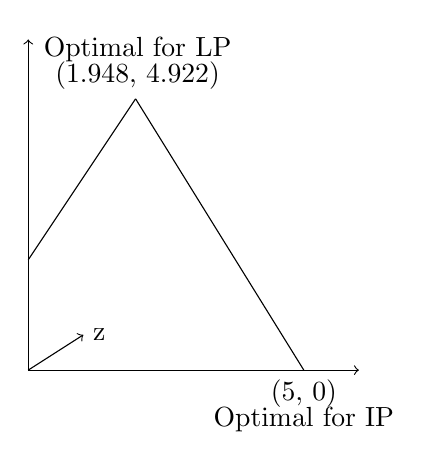
\begin{tikzpicture}[scale=0.7]
						\draw [->] (1,1) -- (1, 7);
						\draw [->] (1,1) -- (7, 1);
						\draw (1,3) -- (2.948, 5.922);
						\draw (2.948, 5.922) -- (6, 1);
						\draw [->] (1,1) -- (2, 1.64);
						\node [right] at (2, 1.64) {z};
						\node [above] at (2.984, 5.922) {(1.948, 4.922)};
						\node [above] at (2.984, 6.422) {Optimal for LP};
						\node [below] at (6,1) {(5, 0)};
						\node [below] at (6, 0.5) {Optimal for IP};
					\end{tikzpicture}
					\caption{Optimal solution for LP / IP}
				\end{figure}

			\subsection{Why Rounding Can be Bad - QAP example}
				Rounding can make the LP useless. For example, for QAP problem, the IP model is
				\begin{align}
					\text{min} \quad z &= \sum_{i\in D} \sum_{s\in O} c_is x_is + \sum_{i\in D} \sum_{j \in D} \sum_{s \in O} \sum_{t\in O} w_{ij}^{st}y_{ij}^{st}  \\
					\text{s.t.} \quad & \sum_{i \in D} x_{is} =1, \quad s\in D  \\
								&\sum_{s \in O} x_{is} = 1, \quad i \in D  \\
								&x_{is} \in \{0, 1\}, \quad i \in D, s\in O  \\
								& y_{ij}^{st} \ge x_{is} + x_{jt} - 1, \quad i\in D, j\in D, s\in O, t \in O  \\
								& y_{ij}^{st} \ge 0, \quad i\in D, j\in D, s\in O, t \in O  \\
								& y_{ij}^{st} \le x_{is}, \quad i\in D, j\in D, s\in O, t \in O  \\
								& y_{ij}^{st} \le x_{jt}, \quad i\in D, j\in D, s\in O, t \in O  
				\end{align}
				We can get the optimal solution for LP supposing $\forall i, s \quad x_{is}\in [0, 1]$
				\begin{align}
					x_{is} &= \frac{1}{|D|}, \quad i \in D, s\in O   \\
					y_{ij}^{st} & = 0, \quad i\in D, j\in D, s\in O, t \in O 
				\end{align}
				
			\subsection{IP and Convex Hull}
				For IP problem
				\begin{align}
					Z_{IP} \quad \text{max} \quad &z = cx  \\
							\text{s.t.} &Ax \le b \\
									&x\in {Z^n} 
				\end{align}
				In feasible region $S = \{x\in Z^n, Ax\le b\}$ , the optimal solution $Z_{IP} = \text{max}\{cx: x\in S\}$.\\
				Denote $conv(S)$ as the convex hull of $S$ then\\
				\begin{equation}Z_{IP}(S) = Z_{IP}(conv(S))  \end{equation}
				
			\subsection{Local Optimal and Global Optimal}
				Let 
				\begin{align}
					Z_s &= \text{min} \{f(x):x\in S\} \\
					Z_t &= \text{min} \{f(x):x\in T\}  \\
					& S \subset T 
				\end{align}
				then\\
				\begin{equation}Z_t \le Z_s  \end{equation}
				\textbf{Notice} that if $x_T^* \in S$ then $x_S^*=x_T^*$, to generalized it, \\
				We have
				\begin{align}
					\begin{cases}x_T^* \in \text{arg min} \{f(x): x\in T\} \\ x_T^* \in S\end{cases} \\ \Rightarrow x_T^*\in \text{arg min} \{f(x): x\in S\} 
				\end{align}
				Especially for IP, we can take the LP relaxation as $T$ and the original feasible region of IP as $S$, therefore, if we find an optimal solution from LP relaxation $T$ which is also a feasible solution of $S$, then it is the optimal solution for IP ($S$)
				
			\subsection{LP Relaxation}
				To perform the LP relaxation, we expand the feasible region
				\begin{align}
					x \in \{0,1\} & \rightarrow x\in [0, 1]  \\
					y\in Z^+ & \rightarrow y \ge 0 
				\end{align}
				If we have $Z_LP(s) = conv(s)$ then
				\begin{equation} LP(s): {x\in R_+^n: Ax\le b}\end{equation}
				The closer $LP(s)$ is to $conv(s)$ the better. Interestingly, we only need to know the convex in the direction of $c$.\\
				There are several formulation problem have the property of $Z_{LP}(s) = conv(s)$, such as:\\
				\indent- Assignment Problem\\
				\indent- Spawning Tree Problem\\
				\indent- Max Flow Problem\\
				\indent- Matching Problem

	\chapter{Decomposition Principle}

	\chapter{Ellipsoid Algorithm}

	\chapter{Projective Algorithm}

	\chapter{Interior-Point Algorithm}